\chapter{Introducción a la optimización convexa}

\columnratio{0.7,0.3}
\begin{paracol}{2}
\section{Introducción}

\begin{tcolorbox}[colback=black!1!white,colframe=white!90!black]
$$
(P)
\left\{
\begin{array}{rl}
    \min & f_0(x)\\\\
    s.a. & f_1(x) \leq b_1\\
	 &f_2(x) \leq b_2\\
	 & \vdots\\
	 & f_m(x) \leq b_m.
\end{array}
\right.
$$
\end{tcolorbox}

Donde,
\switchcolumn[1]*{\noindent \scriptsize
    \begin{itemize}
	\item Las funciones objetivos en economía se les puede llamar funciones de coste.
	\item Multiplicamos las desigualdades por $(-1)$ para darle la forma que más nos convenga darle al problema de optimización.
	\item Maximizar será lo mismo que minimizar. En nuestro caso minimizaremos las funciones. 
	\item Al valor $f_0(x^*)$ se le llamará valor optimo.
	\item En $f_i:  \mathbb{R}^n \rightarrow \mathbb{R}$ existirán algunas funciones el cual su dominio sera "tramposo".
    \end{itemize}
}

\switchcolumn[0]
$$
\begin{array}{rl}
    f_i: & \mathbb{R}^n \rightarrow \mathbb{R}\\
    f_0 : & \mbox{Función objetivo.}\\
    f_j : & \mbox{Función Restricción donde }j=1,\ldots,m.\\
\end{array}
$$

El objetivo de (P) es encontrar $x^*$ el optimo ($\arg\min$) que cumpla:

	    $$f_0(x^*)\leq f_0(x), \;\forall x\in \mathbb{R}^n / f_j(x)\leq b_j,\; j=1,\ldots,m.$$

Los Puntos factibles son los $x\in \mathbb{R}^n / f_j(x)\leq b_j,\; j=1,\ldots,m.$\\

Cuando el problema sea de la forma convexa se llama optimización convexa. Al final, la habilidad es identificar las restricciones y convertirlas a convexas.

\switchcolumn[1]*{\scriptsize
% -------------------- NOTA 1.1
\begin{nota} Imaginemos que tenemos
    $$
    \begin{array}{rl}
	\left\{\min\right. & f(x)\\\\
	\left\{ \min \right. & f_0^2(x)
    \end{array}
    $$
    \begin{itemize}
	\item Si las función $f_0$ es positiva las dos formas son equivalentes. 
	\item El valor optimo no será el mismo, pero el punto optimo lo será, ya que las funciones son monótomas crecientes. 
	\item Si el valor al cuadrado simplificará la solución, entonces podemos utilizarla. Esto nos permite que si no tengamos una función convexa podamos convexificarla.
    \end{itemize}
\end{nota}
}
\switchcolumn[0]\noindent
% -------------------- NOTACIÓN 1.1
\begin{notacion}
    Podemos escribir $Ax$ como
    $$
    \begin{array}{rcl}
	Ax &=& 
	\underset{A^1}{
	\begin{pmatrix}
	    a_{11}\\
	    a_{21}\\
	    \vdots\\
	    a_{k1}
	\end{pmatrix}}
	x_1+
	\underset{A^2}{
	\begin{pmatrix}
		a_{12}\\
		a_{22}\\
		\vdots\\
		a_{k2}
	\end{pmatrix}}
	x_2+
	\cdots +
	\underset{A^n}{
	\begin{pmatrix}
		a_{1n}\\
		a_{2n}\\
		\vdots\\
		a_{kn}
	\end{pmatrix}}
	x_n\\\\
       &=&
	x_1A^1+x_2A^2+\cdots+x_nA^n.
    \end{array}
    $$
    $A^1$ = A super 1 como columna, y $A_1$ = A super 1 como fila.\\

    Ahora, en términos de filas. Si escribimos los vectores A en columna
    $$
    A = 
    \begin{pmatrix}
	    A^T_1\\
	    A^T_2\\
	    \vdots\\
	    A^T_k
    \end{pmatrix}
    $$

    Donde,\\
    $$
    Ax = 
    \begin{pmatrix}
	    A^T_1x\\
	    A^T_2x\\
	    \vdots\\
	    A^T_nx
    \end{pmatrix}
    =
    \begin{pmatrix}
	    \langle A^T_1,x\rangle\\
	    \langle A^T_2,x\rangle\\
	    \vdots\\
	    \langle A^T_n,x\rangle
    \end{pmatrix}
    $$
\end{notacion}


% -------------------- EJEMPLO 1.1 -----------------------------
\begin{ejem}
    Sean $A\in \mathcal{M}_{k\times n},\; \textbf{x}\in \mathbb{R}^n,\; \textbf{b}\in \mathcal{R}^k$.
    $$
    \begin{pmatrix}
	x_1\\
	x_2\\
	\vdots\\
	x_n
    \end{pmatrix}
    \in \mathbb{R}^n,
    \qquad 
    \textbf{x}^T=(x_1,x_2,\ldots,x_n).
    $$
    El problema será una minimización global dada por:\;
    $
    \left\{
    \begin{array}{rl}
	\min: &\|A\textbf{x}-b\|^2_2\\
	s.a. & \emptyset.
    \end{array}
    \right.
    $
\switchcolumn[1]*{\noindent \scriptsize
    \begin{itemize}
	\item Diremos que el un vector cualquiera sera vector columna.
	\item El subindice $_2$ significa la normal Euclidea. Que es la distancia normal que existe en $\mathbb{R}^2.$
    \end{itemize}
}

\switchcolumn[0]
    Solución.-\; Por diferenciabilidad se tiene,
    $$f_0(x)=\|Ax-b\|_2^2 = \langle Ax-b,Ax-b\rangle.$$
    Intentaremos demostrar el punto donde las parciales de $f_0=0$. Para ello, encontraremos 
    $$
    \begin{array}{rcl}
	D_if_0&=&D_i\left(\langle Ax-b, Ax-b\rangle\right)\\\\
	      &=&\langle D_i\left(Ax-b\right),Ax-b\rangle+\langle Ax-b,D_i\left(Ax-b\right)\rangle\\\\
	      &=& 2\langle Ax-b,D_i\left(Ax-b\right)\rangle.
    \end{array}
    $$
    Veamos la parcial de $D_i\left(Ax-b\right)$.
    $$ D_i\left(Ax-b\right)=D_i\left(x_1A^1+x_2A^2+\cdots+x_nA^n-b\right)=A^i.$$
    Dado que $b$ que es constante vale cero, y donde todos los suman que no estén las $x_i$ también valen cero.
    Por lo tanto,
    $$D_if_0 = 2\langle Ax-b,A^i \rangle.$$
    Luego, 
    $$2\langle Ax-b,A^i \rangle = 0 \; \forall i=1,\ldots,n \quad \Rightarrow \quad \langle Ax-b,A^i\rangle=0,\quad \forall i = 1,\ldots,n.$$

\switchcolumn[1]*{\scriptsize
    \begin{itemize}
	\item En funciones convexas el extremo local será el mínimo global.
    \end{itemize}
}
\switchcolumn[0]\noindent
	Observemos que,
	$$
	\overrightarrow{0} = 
	\begin{pmatrix}
	    \langle Ax-b,A^1\rangle\\
	    \langle Ax-b,A^2\rangle\\
	    \vdots\\
	    \langle Ax-b,A^n\rangle
	\end{pmatrix}
	=
	\begin{pmatrix}
	    (A_1)^T\\
	    (A_2)^T\\
	    \vdots\\
	    (A_n)^T
	\end{pmatrix}
	(Ax-b)
	=A^T(Ax-b).
	$$
	$$A^T(Ax-b)=\overrightarrow{0}\quad \Leftrightarrow\quad A^TAx=A^Tb.$$
	El cual es una ecuación normal.

Por último, veamos los argumentos geométricos. Notemos que,
$$\min \|Ax-b\|^2_2 = d(b_i,Ax)^2$$
Donde $Ax$ tendrá la forma geométrica de un subespacio vectorial (en el caso de $\mathbb{R}^3$ será un plano). Entonces,
\switchcolumn[1]*{\noindent
\begin{center}
    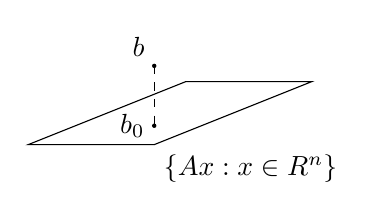
\begin{tikzpicture}[scale=0.4]
      % Define los vértices del romboide
      \coordinate (A) at (0,0);
      \coordinate (B) at (4,0);
      \coordinate (C) at (9,2);
      \coordinate (D) at (5,2);
      % Dibuja el romboide y etiqueta sus vértices
      \draw (A) -- (B) -- (C) -- (D) -- cycle;
      % Que el plano se llame P
      \node [below right] at (B) {$\left\{Ax:x\in \mathbb{R}^n\right\}$};
      % trazar una linea entrecortada perpedicular al plano y los puntos extremos que tengan un punto negro
      \draw[dashed] (4,2.5)node[above left]{$b$} -- (4,.6)node[left]{$b_0$};
      \fill (4,2.5) circle (2pt);
      \fill (4,.6) circle (2pt);
    \end{tikzpicture}
\end{center}
}
\switchcolumn[0]\noindent
    \begin{itemize}
	\item Si $b\in \left\{Ax:x\in \mathbb{R}^n\right\}\; \Leftrightarrow \; x^* \in \mathbb{R}^n : Ax^* =b.$ El valor optimo es $f_0(x^*)=0$.
	\item Si $b\notin \left\{Ax:x\in \mathbb{R}^n\right\}$, $f_0(x^*)=d(b,b_0)^2$.
    \end{itemize}
Ahora, cual es el optimo?; es decir cual es el $x^*$. Para ello, 
$$x^*\in \mathbb{R}^n : Ax^*=b_0.$$ Aquí, $b_0$ está en el plano, si estamos en $\mathbb{R}^3$. ¿Cómo llegamos algebraicamente?:
$$
\begin{array}{rcl}
b-b_0 \perp \left\{Ax:x\in \mathbb{R}^n\right\}&\Leftrightarrow & b-b_o \perp A^i,\; i=1,\ldots,n\\\\  
						 &\Leftrightarrow & \langle b-b_0,A^i\rangle=0,\; i=1,\ldots,n\\\\
							   &\Leftrightarrow& \langle b-Ax^*,A^i\rangle = 0, \; i=1,\ldots,n\\\\
							   &\Leftrightarrow& \langle Ax^*-b,A^i\rangle = 0, \; i=1,\ldots,n\\\\
								   &\Leftrightarrow&A^TAx^*=A^Tb.
\end{array}
$$
(Las ecuaciones normales vienen dadas por la perpendicularidad.)
\end{ejem}

\end{paracol}



\chapter{Conjuntos convexos}

\begin{paracol}{2}

\section{Conjuntos convexos de \boldmath $\mathbb{R}^n$}
El dominio serán conjuntos convexos o dominio efectivo.
\switchcolumn[1]*{\noindent \scriptsize
    \begin{itemize}
	\item Cuando $\lambda$ vale $1$ será $x_1$ cuando valga cero $x_0$. 
	\item Cuando es positivo irá a  la derecha, cuando es negativo hacia la izquierda.
	\item Toda la recta nos da un concepto que denominamos Afín. 
	    Es cualquier punto que este entre $x_0$ y $x_1$ del gráfico de arriba. 
    \end{itemize}
}
\switchcolumn[0]\noindent
    % -------------------- DEFINICIÓN 1 LINEAL
    \begin{def.}[Lineal]\,\\ 
    $$L(x_0,x_1) := \left\{x_0+\lambda(x_1-x_0):\lambda \in \mathbb{R}\right\}$$
    \begin{center}
	\begin{tikzpicture}[scale=0.35]
	  \coordinate (A) at (0,0);
	  \coordinate (B) at (3,1);
	  \coordinate (C) at (6,2);
	  \coordinate (D) at (-3,-1);
	  \draw[->] (A) -- (B)node[below]{$x_1$};
	  \draw[dashed] (B) -- (C);
	  \draw[dashed] (D) -- (A);
	  \fill (A) circle (2pt) node[below]{$x_0$};
	\end{tikzpicture}
    \end{center}
    \end{def.}
    Para la convexidad no es necesario tener la linea, solo necesitaremos un segmento definido por: 
	$$\left[x_0,x_1\right]:=\left\{x_0+\lambda(x_1-x_0):\lambda \in \left[0,1\right]\right\}=\left\{(1-\lambda)x_0+\lambda x_1:\lambda \in \left[0,1\right]\right\}$$

\switchcolumn[1]*{\noindent\scriptsize
    \begin{itemize}
	\item Manejar el concepto de afín con lineas es incomodo, por lo que se utiliza el concepto de combinación afín.
	\item La diferencia entre espacio vectorial y espacio afín es que el espacio afín esta desplazado; es decir, no necesariamente pasa por el cero como en un subespacio vectorial.
    \end{itemize}
}
\switchcolumn[0]\noindent
    % -------------------- DEFINICIÓN 1.2 (AFÍN)
    \begin{def.}
	Sea $A\subseteq \mathbb{R}^n$. Se dice \textbf{Afín}, si $\forall x, y\in A$ se tiene que la $L(x,y)\subseteq A$. (Subespacios vectoriales desplazados).
    \end{def.}

\begin{itemize}
    \item Un circulo no es afín ya que la linea es infinita.
    \item Un plano podría ser Afín.
    \item La recta es afín.
    \item Todo $\mathbb{R}^n$ es afín.
    \item Un único punto también es afín, dado que $x=y$.
\end{itemize}

\switchcolumn[1]*{\noindent\scriptsize
\begin{itemize}
    \item $(1-\lambda)x_0+\lambda x_1$ es una combinación lineal de $x_0$ y $x_1$. Donde $(1-\lambda)+\lambda=1$.
    \item Lo demás puntos fuera del segmento son las combinaciones lineales de $x_0$ y $x_1$.
\end{itemize}
}

\switchcolumn[0]\noindent
% -------------------- DEFINICIÓN 1.3 combinación afín
\begin{def.}
    Una \textbf{combinación afín} de los vectores $\left\{x_1,x_2,\ldots,x_k\right\}$ es un vector de la forma 
$$\lambda_1 x_1+\lambda_2x_2+\cdots+\lambda_kx_k.$$
tal que 
$$\sum_{i=1}^k \lambda_i = 1.$$
\end{def.}

\switchcolumn[1]*{\noindent\scriptsize
    \begin{itemize}
	\item Este conjunto es estable para combinaciones lineales, muy similar al concepto de subespacio vectorial.
    \end{itemize}
}
\switchcolumn[0]\noindent
{\color{blue}
% -------------------- TEOREMA 1.1
    \begin{teo}
    $A$ es afín sii $A$ contiene toda combinación afín de sus puntos.

	Demostración.-\; Primero, tomemos puntos arbitrarios $\left\{x_1,x_2,\ldots,x_k\right\}$ en $A$ tal que 
	$$z=\lambda_1x_1+\lambda_2x_2+\cdots+\lambda_kx_k$$
	donde $\sum\limits_{i=1}^k \lambda_i = 1$. 

	Ahora, consideremos dos puntos $x_i,x_j$ de $z$. Dado que $A$ es afín, entonces $L(x_i,x_j)\subseteq A$, para todo $x_i,x_j$. Esto implica que $z$ está en $A$. Intuitivamente, si 
	$$\lambda_1x_1+\lambda_2 x_2,\quad \lambda_3\lambda_3+\lambda_4\lambda_4,\quad \ldots,\quad  \lambda_{k-1}x_{k-1}+\lambda_kx_k.\qquad \text{con } \sum_{i01}^k y_i=1.$$ 
	están en $A$. Entonces, $z$ tendrá que estar en $A$.

	Para demostrar la otra implicación, tomemos dos puntos cualesquiera $x_1$ e $x_k$ en $A$. Queremos demostrar que 
	$$L(x_1, x_k) = \left\{x_1 + \lambda(x_k - x_1) : \lambda \in \mathbb{R}\right\}$$ 
	está contenido en $A$.
	Por el hecho de que $x_1$ e $x_k$ están en $A$, podemos considerar la línea $L(x_1, x_k)$. Cualquier punto en esta línea se puede expresar como 
	$$z = x_1 + \lambda(x_k - x_1),$$ 
	donde $\lambda \in \mathbb{R}$. Ahora, notemos que $\lambda + (1 - \lambda) = 1$, lo cual es la condición de combinación afín. Y dado que $A$ contiene toda combinación afín de sus puntos, esto implica que $z$ está en $A$. Por lo tanto, $A$ es afín.
    \end{teo}
}
\switchcolumn[1]*{\noindent\scriptsize
% -------------------- NOTA 1.2	
\begin{nota}
La definición de subespacio se refiere a tomar dos escalares y dos vectores, realizar la combinación lineal, donde esta combinación lineal no se saldrá del conjunto dado.
\end{nota}
}
\switchcolumn[0]\noindent
% -------------------- NOTACIÓN 1.2
\begin{notacion}
La suma de Minkowski es la operación de conjuntos; es decir, si $A,E\subseteq \mathbb{R}^n$. Entonces,
$$A=x_0+E=\left\{x_0+e:e\in E \right\} \quad \mbox{o}\quad E=A-x_0=\left\{a-x_0:a\in A\right\}.$$ 
Es sencillamente trasladar los puntos del plano y desplazarlos o moverlos.
\end{notacion}

% -------------------- TEOREMA 1.2
\begin{teo}
    $A\subseteq \mathbb{R}^n$ es afín sii existe un subespacio vectorial $E\subseteq \mathbb{R}^n$ tal que $A=x_0+E$ para todo $x_0\in A$.\\\\
	Demostración.-\; Supongamos que $A$ es afín y fijamos $x_0\in A$. Intentaremos probar que $E=A-x_0$ es un subespacio de $\mathbb{R}^n$, esto es equivalente a decir que:
	$$\lambda,\mu \in \mathbb{R}, e_i,e_2\subseteq E \quad \Rightarrow \quad \lambda e_i+\mu e_2\in E.$$
	Probemos que $\lambda e_1+\mu e_2\in E$; en otras palabras, probaremos que $\lambda e_1+\mu e_2$ es $a-x_0$.
	$$
	\begin{array}{rcl}
	    \lambda e_1+\mu e_2&=&\lambda(a_1-x_0)+\mu(a_2-x_0)\\\\
			       &=&\lambda a_1 + \lambda a_2 - \lambda x_0-\mu x_0\\\\
			       &=&\lambda a_1 + \lambda a_2 - \lambda x_0-\mu x_0 +x_0-x_0\\\\
			       &=&\lambda a_1 + \lambda a_2+(1-\lambda-\mu)x_0-x_0.
	\end{array}
	$$
	Observemos que $\lambda a_1 + \lambda a_2+(1-\lambda-\mu)x_0$ está en $A$, dado a que $\lambda+\mu+(1-\lambda-\mu)=1$. Por lo tanto,
	$$A-x_0=E.$$
	Es un subespacio vectorial.

	Ahora, para demostrar que $A$ es afín, probaré que cualquier combinación afín de elementos de $A$ sigue estando en $A$ (Teorema 1.1).
	Sean,
	$$\left\{a_1,a_2,\ldots,a_k\right\},\; \lambda_1,\lambda_2,\cdots,\lambda_k:\sum \lambda_i=1.$$
	De donde,
	$$
	\begin{array}{rcl}
	    \lambda_1a_1+\lambda_2a_2+\cdots+\lambda_ka_k&=&\lambda_1(e_1-x_0)+\lambda_2(e_2-x_0)+\cdots+\lambda_k(e_k-x_0)\\\\
							   &=& \lambda_1e_1+\cdots+\lambda_ke_k+\left(\displaystyle\sum_{i=1}^k \lambda_i\right)x_0
	\end{array}
	$$
	Observemos que $\lambda_1e_1+\cdots+\lambda_ke_k$ es una combinación lineal afín el cual existe en $E$ y por definición, $\left(\displaystyle\sum_{i=1}^k \lambda_i\right)=1$. Por lo tanto,
	$$E+x_0=A.$$
\end{teo}

% -------------------- DEFINICIÓN 1.4 ENVOLTURA O SPAN AFÍN
\begin{def.}[Envoltura Afín]\,\\\\
    La envolura afín de $B$, $\aff(B)$, es el menor conjunto afín que contiene a $B$. Esto implica que es el conjunto de las combinaciones afines de elementos de $B$ o es la intersección de los conjuntos afines que contienen a $B$ 
\end{def.}

\switchcolumn[1]*{\noindent\scriptsize
\begin{itemize}
    \item Dimensión $0$ un punto.
    \item Dimensión $1$ una recta.
    \item Dimensión $2$ una plano.
\end{itemize}
}

\switchcolumn[0]

% -------------------- DEFINICIÓN 1.5
\begin{def.}
    Si $A$ es Afín se llama "dimensión afín de $A$" a la dimensión de su espacio vectorial.
\end{def.}

% -------------------- EJEMPLO 1.2
\begin{ejem}
    Dado $C\in \mathbb{R}^n$ afín. Siempre existirán una matriz $A\in \mathcal{M}_{p\times n}$ y $b\in \mathbb{R}^p$ tal que
    $$C=\left\{x\in \mathbb{R}^n:Ax=b\right\}.$$\\
	Solución.-\; El conjunto lineal asociado será el núcleo de la aplicación lineal. Es decir,
	$$E=\left\{e\in \mathbb{R}^n:Ae=0\right\},$$
	cualquier solución de $x_0\in C$ de modo que $Ax_0=b$. Tomando un punto de $C$ y otro de $E$, tenemos 
	$$A(x_0+e)=Ax_0+Ae=b+0=b.$$
	Por lo tanto,
	$$C=\left\{x\in \mathbb{R}^n:Ax=b\right\}=x_0+E.$$
	Así, el conjunto afín no es más que el traslado del espacio vectorial.
\end{ejem}

\switchcolumn[1]*{\noindent\scriptsize
\begin{itemize}
    \item El concepto de punto interior es importante, ya que podemos acercarnos al punto $a$ de todas las direcciones. 
    \item Si es un punto relativo interior nos acercaremos por todos los lados del conjunto.
    \item El punto de adherencia o clausura es un punto el cual me puedo acercar de alguna forma.
\end{itemize}
\begin{enumerate}[1)]
    \item En $\mathbb{R}^2$ será un circulo y en $\mathbb{R}^3$ será una esfera.
    \item Son las bolas que están completamente dentro del conjunto. Es decir, no tienen puntos frontera.
    \item Es cualquier bola de $c$ que corta al conjunto o los puntos que contienen a toda su frontera.
    \item El cierre son los puntos interior y los puntos frontera.
    \item Cualquier bola está en el interior cómo en el exterior del conjunto.
    \item Imaginamos un corte transversal para proyectar una imagen. 
\end{enumerate}
}
\switchcolumn[0]\noindent
% -------------------- DEFINICIÓN 2.6
\begin{def.}[Topología de \boldmath$\mathbb{R}^n$]\,\\\\
    Sean $A\subseteq \mathbb{R}^n$ y $a\in \mathbb{R}^n$:
    \begin{enumerate}[1)]
	\item $a\in A$ está en el interior de $A$ $\left(a\in \interior(A) \mbox{ o } a\in \mathring{A} \right)$, cuando existe $\delta>0$ tal que $B(a,\delta)\subseteq A.$
	$$B(a,\delta)=\left\{x\in \mathbb{R}^n:\|x-a\|_2 \leq \delta.\right\}.$$
	\item $A$ se dice abierto si $A=\interior(A)=\mathring{A}.$ 
	\item Decimos que $c\in\mathbb{R}^n$ está en el cierre (o clausura) de $A$, cuando $\exists \left\{a_n\right\}\in A | a_n\to c$ . 
	\item Decimos que $A$ es cerrado cuando $A=\overline{A}$ donde 
	$$\left\{ x\in \mathbb{R}^n: x \mbox{ está en el cierre de A} \right\}.$$
	\item Se llama frontera de $A$, $\partial{A}$ a la intersección $\overline{A}\cap \left( \overline{\mathbb{R}\backslash A}\right)=\overline{A} \backslash \interior(A)$ (Cualquier bola estará una parte en el interior y otra en el exterior del conjunto).
	\item $a\in \relint(A)$ si existe $\delta>0$ tal que $B(a,\delta)\cap Aff(A)\subseteq A$.\\
    \end{enumerate}
\end{def.}


% -------------------- EJEMPLO 2.3
\begin{ejem}
    Dibujemos un plano ($\mathbb{R}^3$)
    \begin{multicols}{2}
    \begin{center}
      \begin{tikzpicture}[scale=0.4]
	\coordinate (A) at (-2,0);
	\coordinate (B) at (6,0);
	\coordinate (C) at (11,3);
	\coordinate (D) at (3,3);
	\draw (A) -- (B) -- (C) -- (D) -- cycle;
	\coordinate (Center) at ($(A)!0.5!(C)$);
	\draw[] ($(Center)+(-1,.5)$) .. controls ($(Center)+(0.2,2)$) and ($(Center)+(3,-.1)$) .. ($(Center)+(1,-.4)$) .. controls ($(Center)+(0,-.5)$) and ($(Center)+(0,-1)$) .. ($(Center)+(-1,-.9)$) .. controls ($(Center)+(-1.5,-1)$) and ($(Center)+(-3,-.5)$) .. ($(Center)+(-1,.5)$);
	\pattern[pattern=north east lines, pattern color=gray!50] ($(Center)+(-1,.5)$) .. controls ($(Center)+(0.2,2)$) and ($(Center)+(3,-.1)$) .. ($(Center)+(1,-.4)$) .. controls ($(Center)+(0,-.5)$) and ($(Center)+(0,-1)$) .. ($(Center)+(-1,-.9)$) .. controls ($(Center)+(-1.5,-1)$) and ($(Center)+(-3,-.5)$) .. ($(Center)+(-1,.5)$);
	\node at ($(Center)+(-.2,.2)$) {\small$B$};
	\node at ($(Center)+(1.9,.7)$) {\small$A$};
      \end{tikzpicture}
    \end{center}
    \begin{itemize}
	\item $B$ es el interior con la frontera.
	\item $A$ es la frontera.
	\item El objetivo será encontrar el punto optimo de un esfera que está proyectada en este plano. 
	\item El conjunto tendrá que ser convexo.
    \end{itemize}
    \end{multicols}
    Veamos algunas propiedades de este conjunto.
    \begin{enumerate}[1)]
	\item $A$ es cerrado | Cualquier punto que ponga en $B$ me puedo acercar por puntos de $B$.
	\item $B$ cerrado.
	\item $\mathring{A}=\emptyset$ | Si yo ponga una bola $\mathbb{R}^3$, se saldrá del conjunto $A$.
	\item $\mathring{B}=\emptyset$ | Ya que no existirá en el plano ninguna esfera. 
	\item $\relint(A)=\emptyset$; $\relint(B)=B\backslash A.$
    \end{enumerate}
\end{ejem}

\switchcolumn[1]*{\noindent\scriptsize
\begin{itemize}
    \item La única diferencia entre combinación convexa y afín es que la combinación convexa es positiva.
\end{itemize}
}
\switchcolumn[0]\noindent
% -------------------- DEFINICIÓN 1.7
\begin{def.}[Combinación convexa]\,\\\\
    Sean $x_1,x_2,\ldots,x_k\in \mathbb{R}^n$ y $\lambda_1,\lambda_2,\ldots,\lambda_k\in \mathbb{R}$ tales que 
    $$\lambda_i\geq 0\; \text{y} \;\displaystyle\sum_{i=1}^{k}\lambda_i=1.$$ 
    Al vector
    $$\sum_{i=1}^{k}\lambda_ix_i=\lambda_1x_1+\lambda_2x_2+\ldots+\lambda_kx_k$$
    se le llama combinación convexa de los puntos $\left\{x_1,\ldots,x_k\right\}$.
\end{def.}

\switchcolumn[1]*{\noindent\scriptsize
\begin{itemize}
    \item En particular, las combinaciones convexas son los segmentos.
\end{itemize}
}
\switchcolumn[0]\noindent
% -------------------- OBSERVACIÓN 1.1
\begin{obs}
    La definición para 2 puntos $\left\{x_1,x_2\right\}$ nos da las combinaciones convexas,
    $$\lambda x_1+(1-\lambda)x_2,\qquad \lambda\geq 0, (1-\lambda)\geq 0 \; \Leftrightarrow \; \lambda \in \left[0,1\right].$$
    Esto es el segmento,
    $$\left\{\lambda x_1+(1-\lambda)x_2: \lambda\in \left[0,1\right]\right\}=\left[x_1,x_2\right].$$
    Nos quedamos con el segmento que los une, eso nos permitirá utilizar las propiedades de los números reales. Por lo que podremos realizar análisis.
\end{obs}

\switchcolumn[1]*{\noindent\scriptsize
\begin{itemize}
    \item Decimos que $C$ es cerrado para las combinaciones convexas. Es decir, no me salgo del conjunto.
\end{itemize}
}
\switchcolumn[0]\noindent
% -------------------- DEFINICIÓN 1.8
\begin{def.}[Convexo]\,\\\\
    Un conjunto $C\in \mathbb{R}^n$ se dice convexo cuando $C$ contiene las combinaciones convexas de sus puntos, si y sólo si
    $$\forall x_1,x_2\in C \Rightarrow \left[x_1,x_2\right]\subseteq C.$$
    Un conjunto es convexo si dados dos puntos el segmento que los une se queda adentro.
\end{def.}

% -------------------- EJEMPLO 1.4
\begin{ejem}\,\\
    \begin{multicols}{3}
	\begin{center}
	  \begin{tikzpicture}[scale=0.8]
	    % Dibuja el contorno del riñón
	    \coordinate (Center) at ($(A)!0.5!(C)$);
	    \draw[] ($(Center)+(-1,.5)$) .. controls ($(Center)+(0.2,2)$) and ($(Center)+(3,-.1)$) .. ($(Center)+(1,-.4)$) .. controls ($(Center)+(0,-.5)$) and ($(Center)+(0,-1)$) .. ($(Center)+(-1,-.9)$) .. controls ($(Center)+(-1.5,-1)$) and ($(Center)+(-3,-.5)$) .. ($(Center)+(-1,.5)$);
	    % Rellena el interior del riñón con líneas
	    \pattern[pattern=north east lines, pattern color=gray!50] ($(Center)+(-1,.5)$) .. controls ($(Center)+(0.2,2)$) and ($(Center)+(3,-.1)$) .. ($(Center)+(1,-.4)$) .. controls ($(Center)+(0,-.5)$) and ($(Center)+(0,-1)$) .. ($(Center)+(-1,-.9)$) .. controls ($(Center)+(-1.5,-1)$) and ($(Center)+(-3,-.5)$) .. ($(Center)+(-1,.5)$);
	    % trazar una linea que una dos puntos del contorno pero este fuere del conjunto
	    \draw[dashed,red](2,-.1)--(3.7,.45);
	    \node at (2.7,-.4) {\small No convexo};
	  \end{tikzpicture}

	  \begin{tikzpicture}[scale=0.7]
	    % Dibuja un óvalo
		\draw (0,0) ellipse (2.5cm and 1.2cm);
		% Agrega un patrón de líneas diagonales al óvalo
		\pattern[pattern=north east lines, pattern color=gray!50] (0,0) ellipse (2.5cm and 1.2cm);
		\node at (0,1.7) {\small Convexo};
	    \end{tikzpicture}

	  \begin{tikzpicture}[scale=0.6]
		\coordinate (A) at (0,0); % Vértice 1
		\coordinate (B) at (2,0); % Vértice 2
		\coordinate (C) at (3,1.73); % Vértice 3
		\coordinate (D) at (2,3.46); % Vértice 4
		\coordinate (E) at (0,3.46); % Vértice 5
		\coordinate (F) at (-1,1.73); % Vértice 6
		\draw (A) -- (B) -- (C) -- (D) -- (E) -- (F) -- cycle; % Dibuja el hexágono
		\draw[pattern=north east lines, pattern color=gray!50] (A) -- (B) -- (C) -- (D) -- (E) -- (F) -- cycle; % Aplica el patrón al hexágono
		\node at (1,4) {\small Convexo};
	    \end{tikzpicture}
	\end{center}
    \end{multicols}
\end{ejem}

Del gráfico 1) ¿Cuál es el menor conjunto convexo que lo contiene?
\begin{center}
  \begin{tikzpicture}[scale=0.8]
    % Dibuja el contorno del riñón
    \coordinate (Center) at ($(A)!0.5!(C)$);
    \draw[red] ($(Center)+(-1,.8)$) .. controls ($(Center)+(0.2,2)$) and ($(Center)+(3,-.1)$) .. ($(Center)+(1,-.5)$) .. controls ($(Center)+(0,-.8)$) and ($(Center)+(0,-1)$) .. ($(Center)+(-1,-.9)$) .. controls ($(Center)+(-1.5,-1)$) and ($(Center)+(-3,-.5)$) .. ($(Center)+(-1,.8)$);
    % Rellena el interior del riñón con líneas
    \pattern[pattern=north east lines, pattern color=gray!50] ($(Center)+(-1,.5)$) .. controls ($(Center)+(0.2,2)$) and ($(Center)+(3,-.1)$) .. ($(Center)+(1,-.4)$) .. controls ($(Center)+(0,-.5)$) and ($(Center)+(0,-1)$) .. ($(Center)+(-1,-.9)$) .. controls ($(Center)+(-1.5,-1)$) and ($(Center)+(-3,-.5)$) .. ($(Center)+(-1,.5)$);
    % trazar una linea que una dos puntos del contorno pero este fuere del conjunto
  \end{tikzpicture}
\end{center}

% ------------------- DEFINICIÓN 1.9
\begin{def.}
    se llama \textbf{envoltura convexa} de $A$ al menor conjunto convexo que lo contiene o a la intersección de todos los convexos que contienen a $A$, denotado por $\co(A)$.
    También es equivalente a decir que
    $$\co(A)=\left\{\mbox{Combinación convexa de puntos de A.}\right\}$$
\end{def.}

{\color{blue}
% ------------------- EJERCICIO 1.1
\begin{ejer}
    Demostrar que la intersección de conjuntos convexos es convexo.\\\\
	Demostración.-\; Demostremos por contradicción. Sean $C_1$ y $C_2$ dos conjuntos convexos. Y sea 
	$$C=C_1\cap C_2.$$
	no convexo. Esto significa que existen $x$ e $y$ tales que 
	$$\left\{\lambda x + (1-\lambda)y:\lambda\in \mathbb{R}\right\}\not\subseteq C.$$ 
	Supongamos ahora que $x$ e $y$ están en $C$. Cómo ambos $C_1$ y $C_2$ son convexos, el segmento definido debe estar en ambos conjuntos. Es decir,
	$$\left\{\lambda x + (1-\lambda)y:\lambda\in \mathbb{R}\right\}\subseteq C.$$ 
	Lo que contradice nuestra suposición inicial. Por lo tanto, $C$ es convexo.
\end{ejer}
}


\switchcolumn[1]*{\noindent\scriptsize
    \begin{itemize}
	\item Contiene los rayos que pasan por el cero e intersecan a un punto dado.
    \end{itemize}
}
\switchcolumn[0]\noindent
% ------------------- DEFINICIÓN 1.10
\begin{def.}[Cono]\,\\\\
    Un conjunto $C\subseteq \mathbb{R}^n$ se llama cono si y sólo si
    $$\lambda x\in C \mbox{ si } x\in C,\; \lambda \geq 0.$$

% ------------------- PROPIEDAD 1
\begin{prop}[Propiedades de los conos]\,
    \begin{enumerate}[\bfseries a)]
	\item Un cono siempre contiene al origen.
	\item La envoltura cónica de un conjunto es $\con(A)=\left\{\lambda : \lambda \geq 0, a\in A\right\}$. La intersección de todos los conos que contiene a $A$.
	\item Un cono $C$ es convexo si y sólo si 
	$$\lambda_1,\lambda_2\in C \Rightarrow \lambda_1x_1+\lambda_2x_2\in C, \; \forall \lambda_1,\lambda_2 \geq 0.$$
    \item $C$ es un cono convexo si 
    $$\sum_{i=1}^m \lambda_ix_i\in C$$
    para $\lambda_i\geq 0.$
    \end{enumerate}
\end{prop}
\end{def.}

\

\switchcolumn[1]*{\noindent\scriptsize
\begin{itemize}
    \item El hiperplano es un caso particular del estudio convexo.
    \item Hiperplano:
    \begin{center}
	\begin{tikzpicture}[scale=0.4,>=Triangle]
	  \coordinate (A) at (0,0);
	  \coordinate (B) at (4,0);
	  \coordinate (C) at (9,2);
	  \coordinate (D) at (5,2);
	  \draw (A) -- (B) -- (C) -- (D) -- cycle;
	  \node [below right] at (B) {$H$};
	  \draw[<-](4,2.5)node[above left]{$a$} -- (4,.6);
	  \fill (4,2.5) circle (2pt);
	  \fill (4,.6) circle (2pt);
	\end{tikzpicture}
    \end{center}
    \item En $\mathbb{R^2}$ los hiperplanos son rectas.
    \item En $\mathbb{R}^n$, los hiperplanos serán uno menos de dimensión.
\end{itemize}
}
\switchcolumn[0]\noindent
% ------------------- DEFINICIÓN 2.11
\begin{def.}[Hiperplano]\,\\\\
    $H\subseteq \mathbb{R}^n$ es un \textbf{hiperplano} si existe $a\in \mathbb{R}^n \backslash\left\{0\right\}$ tal que
    $$H=\left\{x\in \mathbb{R}^n : \langle a,x\rangle = a^T x = 0\right\} = a^\perp.$$
\end{def.}

{\color{blue}
%------------------- PROPOSICIÓN 2.1
\begin{proposicion}
    $H\subseteq \mathbb{R}^n$ es un hiperplano si y sólo si, $H$ es un subespacio de dimensión $n-1$.\\\\
	Demostración.-\; Primero, supongamos que $H$ es un hiperplano. Entonces, por definición, existe un vector $a \in \mathbb{R}^n \setminus \{0\}$ tal que 
	$$H = \left\{x \in \mathbb{R}^n : a^T x = 0\right\}=a^{\perp}$$ 
	Esto significa que $H$ es el conjunto de todos los vectores que son ortogonales a $a$. Recordemos que cualquier múltiplo escalar del primer vector también es ortogonal al segundo; además, si dos vectores son ortogonales a otro, entonces la suma de los dos primeros vectores también será ortogonal al tercer vector. Es decir, la ortogonalidad preserva las operaciones de suma y multiplicación por escalares. Por lo tanto, $H$ es un subespacio de $\mathbb{R}^n$. Ahora bien, como $a$ no es el vector cero, el conjunto $\{a\}$ es linealmente independiente (ya que no hay otros vectores), y por lo tanto forma una base para un subespacio de $\mathbb{R}^n$. Como este subespacio es ortogonal a $H$, la dimensión de $H$ debe ser $n - 1$.

	Ahora supongamos que $H$ es un subespacio de $\mathbb{R}^n$ de dimensión $n - 1$. Entonces, existe un subespacio de $\mathbb{R}^n$ que es ortogonal a $H$ y tiene dimensión $1$. Este subespacio tiene una base formada por un único vector, digamos $a$. Entonces, para cualquier vector $x \in H$, tenemos que $a^T x = 0$, lo que significa que $x$ es ortogonal a $a$. Por lo tanto, podemos escribir $H = \{x \in \mathbb{R}^n : a^T x = 0\}$, lo que significa que $H$ es un hiperplano.
\end{proposicion}
}

\switchcolumn[1]*{\noindent\scriptsize
\begin{center}
    \begin{tikzpicture}[scale=0.4,>=Triangle]
	\draw[rotate around={70:(0,0)}] (0,0) ellipse (2.5cm and 1.2cm);
	\pattern[pattern=north east lines, pattern color=gray!50, rotate around={70:(0,0)}] (0,0) ellipse (2.5cm and 1.2cm);
	\draw (1,-4) -- (3,3);
	\draw (2,-4) -- (4,3);
	\fill (3,-0.5) circle (4pt) node[above]{$0$};
	\draw (3,-4) -- (5,3);
    \end{tikzpicture}
\end{center}
\begin{itemize}
    \item Un hiperplano en $\mathbb{R}^2$ será sencillamente las rectas.
    \item Esa recta me va a definir dos semiespacios uno al lado del otro.
    \item Nos interesará desplazar esa recta que contiene al $0$. 
    \item La $b$ nos dará una notación de distancia entre los hiperplanos.
\end{itemize}
}
\switchcolumn[0]\noindent
Observemos que la recta que pasa por el cero estará definida por:
    $$\left\{x\in \mathbb{R}^n : \langle a,x\rangle = a^T x = 0\right\} = a^\perp.$$
Y todos los hiperplanos que serán paralelos a esa recta estarán dadas por:
$$\left\{x\in \mathbb{R}^n : \langle a,x\rangle = a^T x = b\right\}.$$
 Esto, nos dará dos semiespacios dados por:
$$\left\{x\in \mathbb{R}^n : a^Tx\leq b\right\}$$
$$\left\{x\in \mathbb{R}^n : a^Tx > b\right\}$$
Esto nos divide el espacio en dos trozos. Que es la estrategia fundamental de análisis de datos. Por ejemplo cuando marcamos con lineas cuando existen datos por arriba y por abajo.

%------------------- EJEMPLO 1.5
\begin{ejem}\,
    \begin{center}
	\begin{tikzpicture}[scale=1,>=Triangle]
	    \fill (0,3) circle (2pt);
	    \draw[dashed] (0,5) -- (2,2)node[below]{$a^Tx=0$};
	    \draw[->] (1,3.5) -- (2,4.2);
	    \fill (1,3.5) circle (1.5pt) node[below left]{\small$0$};
	    \draw (1,6) -- (3,3)node[below]{$a^Tx=b$};
	    \fill (1.66,5) circle (1.7pt)node[left]{$x$};
	    \fill (2.6,3.6) circle (1.7pt)node[left]{$x_0$};
	    \draw[->,green] (2.6,3.6) -- (1.66,5);
	    \draw[->] (2.6,3.6) -- (3.5,4.2);
	    \draw (3.2,3.9)node[below]{\small$a$};
	\end{tikzpicture}
    \end{center}
    Para decidir en que dirección estará el punto, debemos tomar en cuenta a que lado apunto $a$, que nos marcará un punto perpendicular a ese conjunto. De donde,
    $$\langle (x-x_0), a\rangle = 0.$$
    Si queremos en producto matricial se tiene,
    $$
    \begin{array}{rcl}
	a^T(x-x_0)&=&0\\\\
	a^Tx-a^Tx_0&=&0\\\\
	a^Tx&=&a^Tx_0\\\\
	a^Tx &=& b
    \end{array}
    $$
\end{ejem}

\switchcolumn[1]*{\noindent\scriptsize
    \begin{itemize}
	\item Estas aplicaciones la llaman también aplicaciones del dual.
    \end{itemize}
}
\switchcolumn[0]\noindent
%------------------- EJEMPLO 1.6
\begin{ejem}\,
    \begin{center}
	\begin{tikzpicture}[scale=1, >=Triangle]
	    \pattern[pattern=north east lines, pattern color=gray!35, rotate around={34:(1,6)}] (1,6) rectangle (2.5cm,2.4cm);
	    \fill (0,3) circle (2pt);
	    \draw[dashed] (0,5) -- (2,2);
	    \draw[->] (1,3.5) -- (2,4.2);
	    \fill (1,3.5) circle (1.5pt) node[below left]{\small$0$};
	    \draw (1,6) -- (3,3)node[below]{$a^Tx=b$};
	    \fill (2.7,5) circle (1.7pt)node[left]{$x$};
	    \fill (2.6,3.6) circle (1.7pt)node[left]{$x_0$};
	    \draw[->,green] (2.6,3.6) -- (2.7,5);
	    \draw[->] (2.6,3.6) -- (3.5,4.2);
	    \draw (3.2,3.9)node[below]{\small$a$};
	    \draw (2,6.5)node[below]{$H^+$};
	    \draw (.7,5.5)node[below]{$H^-$};
	\end{tikzpicture}
    \end{center}
    El angulo de $(x-x_0,a)$ esta entre $-90^\circ$ y $90^\circ$. En términos de cosenos sería:
    $$\cos\left[\text{ang}(x-x_0,a)\right]\in [0,1]$$
    Luego, 
    $$0\leq \cos\left[\text{ang}(x-x_0,a)\right]=\frac{\langle (x-x_0),a\rangle}{\|x-x_0\|_2\|a\|_2}$$
    Por lo tanto,
    $$
    \begin{array}{rcl}
	x\in H^+ &\Leftrightarrow& \langle (x-x_0),a\rangle = \cos\left[\text{ang}(x-x_0),a\right]\|x-x_0\|_2\|a\|_2 \geq 0\\\\
		 &\Leftrightarrow& \langle (x-x_0),a\rangle \geq 0\\\\
		 &\Leftrightarrow& \langle x,a\rangle \geq \langle x_0,a\rangle\\\\
		 &\Leftrightarrow& a^Tx\geq a^Tx_0\\\\
		 &\Leftrightarrow& a^Tx\geq b
    \end{array}
    $$
    Ahora, si $x\in H^-$, entonces $a^Tx\leq b$.
\end{ejem}


\section{Bolas Euclideas}

\switchcolumn[1]*{\scriptsize
\begin{center}
    \begin{tikzpicture}[scale=.55,line cap=round, line join=round, >=Triangle]
      \clip(-2.19,-2.49) rectangle (2.66,2.58);
      \draw(0,0) circle (2cm);
      \draw [rotate around={0.:(0.,0.)},dash pattern=on 3pt off 3pt] (0,0) ellipse (2cm and 0.9cm);
      \draw [rotate around={0.:(0.,0.)},dash pattern=on 3pt off 3pt] (0,0) ellipse (0.9cm and 2cm);
      \draw[->](0,0)-- (0.70,1.07);
      \draw [->,gray!50] (0,0) -- (0,2);
      \draw [->,gray!50] (0,0) -- (-0.81,-0.79);
      \draw [->,gray!50] (0,0) -- (2,0);
      \draw [dotted] (0.7,1)-- (0.7,-0.46);
      \draw [dotted] (0,0)-- (0.7,-0.46);
      \draw (0.9,1.3) node[] {$a$};
    \end{tikzpicture}
\end{center}
}
\switchcolumn[0]\noindent
Tenemos que,
$$
\begin{array}{rcl}
    B(c,r)&=&\left\{x\in \mathbb{R}^n : \|x-c\|_2<r\right\}\\\\
	  &=& \left\{x\in \mathbb{R}^n : (x-c)^T(x-c)<r^2\right\}.
\end{array}
$$

{\color{blue}
%------------------- EJERCICIO 1.2
\begin{ejer}
    Demostrar que $B(c,r)$ es convexo.\\\\
	Demostración.-\; Sean $x_0,x_1$ en $B(c,r)$ y $\lambda\in[0,1]$. Demostraremos que 
	$$(1-t)x_0+\lambda x_1$$
	esta también en $B(c,r)$. Primero, notemos que 
	$$\|x_0-c\|_2<r \quad \text{y}\quad \|x_1-c\|_2<r.$$
	Luego, por la definición de convexidad, y por la desigualdad triangular,
	$$
	\begin{array}{rcl}
	    \|\left[(1-\lambda)x_0+\lambda x_1\right]-c\|_2&=&\|\lambda(x_0-c)+(1-\lambda)(x_1-c)\|_2\\\\
					      &\leq& \lambda\|x_0-c\|_2+(1-\lambda)\|x_1-c\|_2\\\\
					      &<& \lambda r+(1-\lambda)r.
	\end{array}
	$$
	Por lo tanto,
	$$\|(1-\lambda)x_0+\lambda x_1-c\|_2<r.$$
	Concluimos que, $B(r,c)$ es convexo. (La demostración se basó en el libro de Boyd).
\end{ejer}
}

\switchcolumn[1]*{\noindent\scriptsize
    \begin{itemize}
	\item Si la bola está al rededor del cero u otro punto, la bola es la misma. Esto en distancias no tiene porque ser cierto.
	\item Todas las bolas que podamos dibujar podremos representarlos con centro cero, ya sean grandes o pequeñas.
    \end{itemize}
}
\switchcolumn[0]\noindent
%------------------- PROPIEDAD 2
\begin{prop}
    Mediante la suma de Minskowsky tenemos,
    $$B(c,r)=c+rB(0,r).$$
\end{prop}

\section{Elipsoides}

\switchcolumn[1]*{\scriptsize
    \begin{itemize}
	\item Cómo es simétrica y tiene valores propios positivos, se puede utilizar la diagonalización y escribir la matriz $P$ cómo producto de una matriz diagonal por dos matrices de cambio que en realidad son ortonormales.
	\item $z^TDz$, se puede hacer más grande o mas pequeña.
	\item Los vectores de $L$ me dan los vectores que apuntan a la elipse.
	\item $z^TDz$ es el circulo.
	\item $D$ serán las curvaturas principales de la elipse.
	\item La $L$ gira la elipsoide.
	\item Los elipsiodes se manejan para manejar imagenes donde incluye un objeto.
    \end{itemize}
}
\switchcolumn[0]\noindent
$$
\begin{array}{rcllc}
    \mathcal{E}&=&\left\{x\in \mathbb{R}^n : (x-c)^TP^{-1} (x-c)\leq 1\right\}&&(1)\\\\
	       &=& c+\left\{y\in \mathbb{R}^n : y^r P^{-1} y \leq 1\right\} & (y=x-c)&(2)\\\\
	       &=&c+\left\{y\in \mathbb{R}^n : y^T L D L^T y \leq 1\right\}&&(3)\\\\
	       &=&c+\left\{Lz : z^T D z \leq 1\right\} & (z=L^Ty)&(4)\\\\
	       &=& c+L\left\{z:z^TDz\leq 1\right\}. &&(5)
\end{array}
$$
donde 
$$P=P^T>0 \text{ (Simétrica y valores propios}>0).$$
y
$$P^{-1}=LDL^T,\; \text{Si } P\in \mathcal{M}_{n\times n}.$$
donde $D$ es una matriz diagonal con valores propios de $1/P$.

\begin{center}
\begin{tikzpicture}[rotate=45, >=Triangle,scale=.6]
    \draw (0,0)node[below]{\small$c$} ellipse (2cm and 1cm);
    \draw[->] (0,0) -- node[above]{\tiny$L$} (2,0);
    \draw[->] (0,0) -- node[above]{\tiny$L$} (0,1);
    \draw(-2,-1)node[below]{\small$(1)$};

    \draw (2,-2)node[above]{\small$\Rightarrow$};

    \draw (4,-4)node[below left]{\small$0$} ellipse (2cm and 1cm);
    \draw[->] (4,-4) -- node[above]{\tiny$L$} (6,-4);
    \draw[->] (4,-4) -- node[above]{\tiny$L$} (4,-3);
    \draw(1.5,-4)node[below]{\small$(3)$};

    \draw[rotate=-45,color=green] (5.7,0) ellipse (2cm and 1cm);
    \draw[color=green](6,-5.7)node[below]{\small$(5)$};
    \draw[->,rotate=-45,color=green] (5.7,0) -- node[above]{\tiny$L$} (7.7,0);
    \draw[->,rotate=-45,color=green] (5.7,0) -- node[above]{\tiny$L$} (5.5,-1);
\end{tikzpicture}
\end{center}


\section{Bolas generales y conos asociados}
%------------------- DEFINICION 2.12
\begin{def.}[Norma] $\|\cdot\|:\mathbb{R}^n\to \mathbb{R}^+.$

Algunas condiciones:
\begin{enumerate}[\bfseries i)]
    \item $\|x\|=0 \Leftrightarrow x=0.$
    \item Si la norma de un vector se eleva al cuadrado, se esperara que la longitud sea el doble. 
	$$\|\lambda x\|=|\lambda|\|x\| \quad \forall \lambda \in \mathbb{R}.$$
    \item La desigualdad triangular.
	$$\|x+y\|\leq \|x\|+\|y\|.$$
\end{enumerate}
\end{def.}

Recordemos que,

$$
\begin{array}{rcl}
    B(c,r)&=&\left\{x\in \mathbb{R}^n : \|x-c\|\leq r\right\}\\\\
	  &=&\left\{x\in \mathbb{R}^n : d_{\|\cdot\|}(x,c)\leq r\right\}.
\end{array}
$$

Donde $B(c,r)$ es convexa.

\subsection{Cono asociado a una norma}


\switchcolumn[1]*{\noindent\scriptsize
    \begin{itemize}
	\item Una vez que conoces la $B(0,1)$ se conoce todas las demás.
	\item No se puede derivar en el origen, ya que estará en el pico del cono.
	\item Podemos analizar todo lo que está dentro del cono,
	\item A esto se le llama epigrafo de la función, es decir dibujar la función y pintar todo lo que hay arriba. 
	\item La definición del cono es cerrada.
    \end{itemize}
}
\switchcolumn[0]\noindent
%------------------- DEFINICION 2.13
\begin{def.}
    $$C_{\|\cdot\|}=\left\{(x,t)\in \mathbb{R}^n \times \mathbb{R} : \|x\|\leq t\right\}.$$
\begin{center}
    \begin{tikzpicture}[scale=0.8,>=Triangle]
      \draw(-2.5,-1.5) -- (1.8,-1.5) -- (2.8,-.7);
      \draw(3.2,-1.5)node[above]{\small$B(0,1)$};
      \draw[dashed](2.8,-.7) -- (-1.5,-.7);
      \draw(-1.5,-.7) -- (-2.5,-1.5);
      \draw[opacity=.7] (0,-1.05) ellipse (.67cm and 0.2cm);
	\draw[opacity=.5](0,0) ellipse (1.5cm and 0.3cm);
	\draw[<-] (-1.5,0) -- (0,-2);
	\draw[<-] (1.5,0) -- (0,-2);
	\draw[opacity=.4] (0,-2) ellipse (.67cm and .2cm); % elipse en la base
	\draw[opacity=.3] (-1.5,-2) -- (1.5,-2); % recta horizontal
	\draw[opacity=.3] (-.7,-2.5) -- (.6,-1.6); % recta vertical
    \end{tikzpicture}
\end{center}

$$\left\{(x,t):t=1\cap C_{\|\cdot\|}\right\}=\overline{B(x,t)}.$$
\end{def.}

\subsubsection{Tipos de norma}
\begin{enumerate}[\bfseries a)]
    \item $\|\cdot\|_1:\mathbb{R}^2\to \mathbb{R}$, $\|(x,y)\|_1=|x|+|y|.$ Si lo definimos en $\mathbb{R}^8$ las sumas serán la suma de sus componentes. Si queremos dibujar $\overline{B(0,1)}$
    \begin{center}
	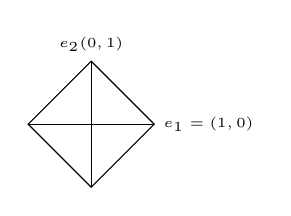
\begin{tikzpicture}[scale=.4]
	    \draw (-.5,0) -- (1.5,2) -- (3.5,0) -- (1.5,-2) -- cycle; % Dibuja el rombo
	    \draw (-.5,0) -- (3.5,0)node[right]{\tiny$e_1=(1,0)$}; % Dibuja la línea horizontal
	    \draw (1.5,2)node[above]{\tiny$e_2(0,1)$} -- (1.5,-2); % Dibuja la línea vertical
	\end{tikzpicture}
    \end{center}
    Donde, $e_1$ y $e_2$ se llaman extremales.

\begin{center}
    \begin{tikzpicture}[scale=0.8,>=Triangle]
      \draw(-2.5,-1.5) -- (1.8,-1.5) -- (2.8,-.7);
      \draw(3.2,-1.5)node[above]{\small$B(0,1)$};
      \draw[dashed](2.8,-.7) -- (-1.5,-.7);
      \draw(-1.5,-.7) -- (-2.5,-1.5);
	\draw[<-] (-1.5,0) -- (0,-2);
	\draw[<-] (1.5,0) -- (0,-2);
	\draw[<-] (-.3,-.5) -- (0,-2);
	\draw[<-,dashed] (.5,.4) -- (0,-2);
	\draw[opacity=.5](-1.5,0) -- (.5,.4) -- (1.5,0) -- (-.3,-.5) -- cycle;
	\draw[opacity=.5](-.75,-1) -- (0.25,-.8) -- (.75,-1) -- (-.15,-1.3) -- cycle;
	\draw[opacity=.3] (-1.5,-2) -- (1.5,-2); % recta horizontal
	\draw[opacity=.3] (-.7,-2.5) -- (.6,-1.6); % recta vertical
    \end{tikzpicture}
\end{center}
\item $\|\cdot\|_\infty: \mathbb{R}^n\to \mathbb{R}$, $\|x,y\|_\infty=\max\left\{|x|,|y|\right\}$. Compara y coge la más grande.
\end{enumerate}



\end{paracol}
